% Graphic for TeX using PGF
% Title: D:\Dokumente\GitHub\Bachelorarbeit\Arbeitstagebuch\src\04.07.2017-RPNTree-classdiagram.dia
% Creator: Dia v0.97.2
% CreationDate: Wed Aug 30 19:22:10 2017
% For: Timo Bergerbusch
% \usepackage{tikz}
% The following commands are not supported in PSTricks at present
% We define them conditionally, so when they are implemented,
% this pgf file will use them.
\ifx\du\undefined
  \newlength{\du}
\fi
\setlength{\du}{15\unitlength}
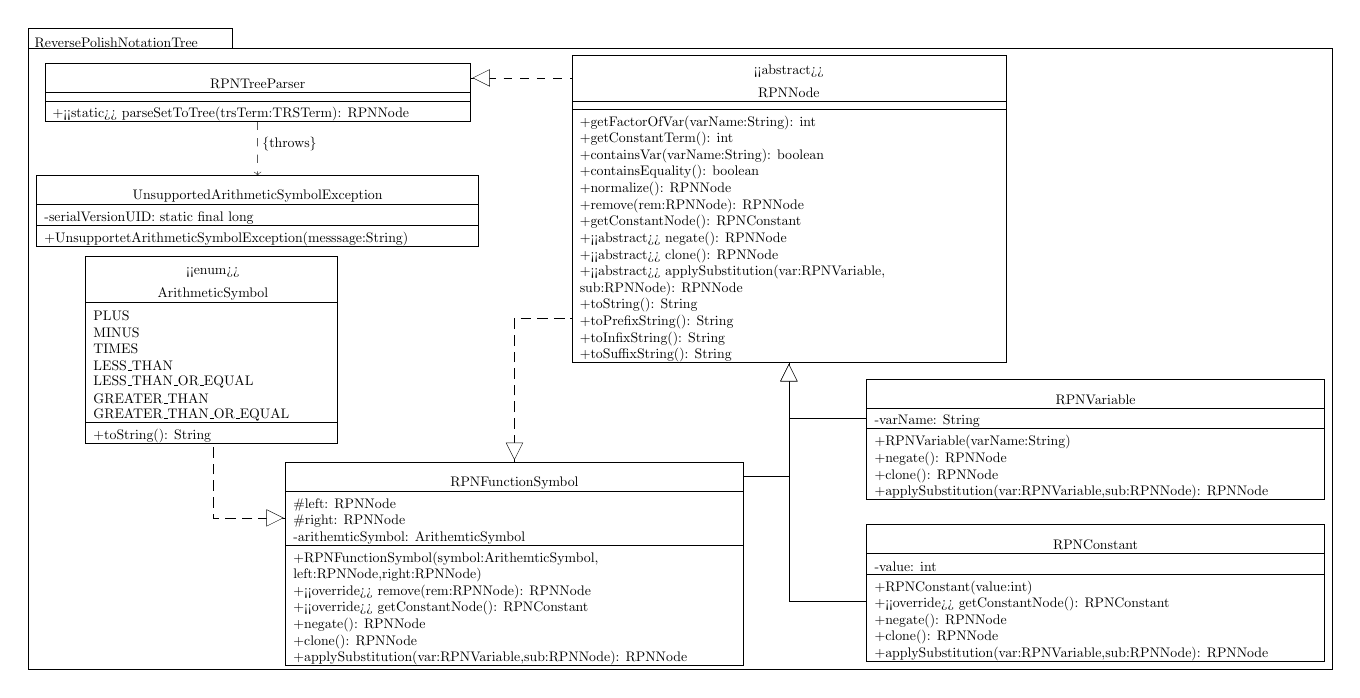
\begin{tikzpicture}[scale=0.5, every node/.style={scale=0.5}]
\pgftransformxscale{1.000000}
\pgftransformyscale{-1.000000}
\definecolor{dialinecolor}{rgb}{0.000000, 0.000000, 0.000000}
\pgfsetstrokecolor{dialinecolor}
\definecolor{dialinecolor}{rgb}{1.000000, 1.000000, 1.000000}
\pgfsetfillcolor{dialinecolor}
\pgfsetlinewidth{0.010000\du}
\pgfsetdash{}{0pt}
\definecolor{dialinecolor}{rgb}{1.000000, 1.000000, 1.000000}
\pgfsetfillcolor{dialinecolor}
\fill (-2.412990\du,34.090900\du)--(-2.412990\du,64.000000\du)--(60.422652\du,64.000000\du)--(60.422652\du,34.090900\du)--cycle;
\definecolor{dialinecolor}{rgb}{0.000000, 0.000000, 0.000000}
\pgfsetstrokecolor{dialinecolor}
\draw (-2.412990\du,34.090900\du)--(-2.412990\du,64.000000\du)--(60.422652\du,64.000000\du)--(60.422652\du,34.090900\du)--cycle;
\definecolor{dialinecolor}{rgb}{1.000000, 1.000000, 1.000000}
\pgfsetfillcolor{dialinecolor}
\fill (-2.412990\du,33.090900\du)--(-2.412990\du,34.090900\du)--(7.412010\du,34.090900\du)--(7.412010\du,33.090900\du)--cycle;
\definecolor{dialinecolor}{rgb}{0.000000, 0.000000, 0.000000}
\pgfsetstrokecolor{dialinecolor}
\draw (-2.412990\du,33.090900\du)--(-2.412990\du,34.090900\du)--(7.412010\du,34.090900\du)--(7.412010\du,33.090900\du)--cycle;
% setfont left to latex
\definecolor{dialinecolor}{rgb}{0.000000, 0.000000, 0.000000}
\pgfsetstrokecolor{dialinecolor}
\node[anchor=west] at (-2.312990\du,33.790900\du){ReversePolishNotationTree};
\pgfsetlinewidth{0.010000\du}
\pgfsetdash{}{0pt}
\definecolor{dialinecolor}{rgb}{1.000000, 1.000000, 1.000000}
\pgfsetfillcolor{dialinecolor}
\fill (23.800000\du,34.400000\du)--(23.800000\du,36.600000\du)--(44.705000\du,36.600000\du)--(44.705000\du,34.400000\du)--cycle;
\definecolor{dialinecolor}{rgb}{0.000000, 0.000000, 0.000000}
\pgfsetstrokecolor{dialinecolor}
\draw (23.800000\du,34.400000\du)--(23.800000\du,36.600000\du)--(44.705000\du,36.600000\du)--(44.705000\du,34.400000\du)--cycle;
% setfont left to latex
\definecolor{dialinecolor}{rgb}{0.000000, 0.000000, 0.000000}
\pgfsetstrokecolor{dialinecolor}
\node at (34.252500\du,35.160000\du){<<abstract>>};
% setfont left to latex
\definecolor{dialinecolor}{rgb}{0.000000, 0.000000, 0.000000}
\pgfsetstrokecolor{dialinecolor}
\node at (34.252500\du,36.200000\du){RPNNode};
\definecolor{dialinecolor}{rgb}{1.000000, 1.000000, 1.000000}
\pgfsetfillcolor{dialinecolor}
\fill (23.800000\du,36.600000\du)--(23.800000\du,37.000000\du)--(44.705000\du,37.000000\du)--(44.705000\du,36.600000\du)--cycle;
\definecolor{dialinecolor}{rgb}{0.000000, 0.000000, 0.000000}
\pgfsetstrokecolor{dialinecolor}
\draw (23.800000\du,36.600000\du)--(23.800000\du,37.000000\du)--(44.705000\du,37.000000\du)--(44.705000\du,36.600000\du)--cycle;
\definecolor{dialinecolor}{rgb}{1.000000, 1.000000, 1.000000}
\pgfsetfillcolor{dialinecolor}
\fill (23.800000\du,37.000000\du)--(23.800000\du,49.200000\du)--(44.705000\du,49.200000\du)--(44.705000\du,37.000000\du)--cycle;
\definecolor{dialinecolor}{rgb}{0.000000, 0.000000, 0.000000}
\pgfsetstrokecolor{dialinecolor}
\draw (23.800000\du,37.000000\du)--(23.800000\du,49.200000\du)--(44.705000\du,49.200000\du)--(44.705000\du,37.000000\du)--cycle;
% setfont left to latex
\definecolor{dialinecolor}{rgb}{0.000000, 0.000000, 0.000000}
\pgfsetstrokecolor{dialinecolor}
\node[anchor=west] at (23.950000\du,37.660000\du){+getFactorOfVar(varName:String): int};
% setfont left to latex
\definecolor{dialinecolor}{rgb}{0.000000, 0.000000, 0.000000}
\pgfsetstrokecolor{dialinecolor}
\node[anchor=west] at (23.950000\du,38.460000\du){+getConstantTerm(): int};
% setfont left to latex
\definecolor{dialinecolor}{rgb}{0.000000, 0.000000, 0.000000}
\pgfsetstrokecolor{dialinecolor}
\node[anchor=west] at (23.950000\du,39.260000\du){+containsVar(varName:String): boolean};
% setfont left to latex
\definecolor{dialinecolor}{rgb}{0.000000, 0.000000, 0.000000}
\pgfsetstrokecolor{dialinecolor}
\node[anchor=west] at (23.950000\du,40.060000\du){+containsEquality(): boolean};
% setfont left to latex
\definecolor{dialinecolor}{rgb}{0.000000, 0.000000, 0.000000}
\pgfsetstrokecolor{dialinecolor}
\node[anchor=west] at (23.950000\du,40.860000\du){+normalize(): RPNNode};
% setfont left to latex
\definecolor{dialinecolor}{rgb}{0.000000, 0.000000, 0.000000}
\pgfsetstrokecolor{dialinecolor}
\node[anchor=west] at (23.950000\du,41.660000\du){+remove(rem:RPNNode): RPNNode};
% setfont left to latex
\definecolor{dialinecolor}{rgb}{0.000000, 0.000000, 0.000000}
\pgfsetstrokecolor{dialinecolor}
\node[anchor=west] at (23.950000\du,42.460000\du){+getConstantNode(): RPNConstant};
% setfont left to latex
\definecolor{dialinecolor}{rgb}{0.000000, 0.000000, 0.000000}
\pgfsetstrokecolor{dialinecolor}
\node[anchor=west] at (23.950000\du,43.260000\du){+<<abstract>> negate(): RPNNode};
% setfont left to latex
\definecolor{dialinecolor}{rgb}{0.000000, 0.000000, 0.000000}
\pgfsetstrokecolor{dialinecolor}
\node[anchor=west] at (23.950000\du,44.060000\du){+<<abstract>> clone(): RPNNode};
% setfont left to latex
\definecolor{dialinecolor}{rgb}{0.000000, 0.000000, 0.000000}
\pgfsetstrokecolor{dialinecolor}
\node[anchor=west] at (23.950000\du,44.860000\du){+<<abstract>> applySubstitution(var:RPNVariable,};
\definecolor{dialinecolor}{rgb}{0.000000, 0.000000, 0.000000}
\pgfsetstrokecolor{dialinecolor}
\node[anchor=west] at (23.950000\du,45.660000\du){                                sub:RPNNode): RPNNode};
% setfont left to latex
\definecolor{dialinecolor}{rgb}{0.000000, 0.000000, 0.000000}
\pgfsetstrokecolor{dialinecolor}
\node[anchor=west] at (23.950000\du,46.460000\du){+toString(): String};
% setfont left to latex
\definecolor{dialinecolor}{rgb}{0.000000, 0.000000, 0.000000}
\pgfsetstrokecolor{dialinecolor}
\node[anchor=west] at (23.950000\du,47.260000\du){+toPrefixString(): String};
% setfont left to latex
\definecolor{dialinecolor}{rgb}{0.000000, 0.000000, 0.000000}
\pgfsetstrokecolor{dialinecolor}
\node[anchor=west] at (23.950000\du,48.060000\du){+toInfixString(): String};
% setfont left to latex
\definecolor{dialinecolor}{rgb}{0.000000, 0.000000, 0.000000}
\pgfsetstrokecolor{dialinecolor}
\node[anchor=west] at (23.950000\du,48.860000\du){+toSuffixString(): String};
\pgfsetlinewidth{0.010000\du}
\pgfsetdash{}{0pt}
\definecolor{dialinecolor}{rgb}{1.000000, 1.000000, 1.000000}
\pgfsetfillcolor{dialinecolor}
\fill (38.000000\du,50.000000\du)--(38.000000\du,51.400000\du)--(60.060000\du,51.400000\du)--(60.060000\du,50.000000\du)--cycle;
\definecolor{dialinecolor}{rgb}{0.000000, 0.000000, 0.000000}
\pgfsetstrokecolor{dialinecolor}
\draw (38.000000\du,50.000000\du)--(38.000000\du,51.400000\du)--(60.060000\du,51.400000\du)--(60.060000\du,50.000000\du)--cycle;
% setfont left to latex
\definecolor{dialinecolor}{rgb}{0.000000, 0.000000, 0.000000}
\pgfsetstrokecolor{dialinecolor}
\node at (49.030000\du,51.000000\du){RPNVariable};
\definecolor{dialinecolor}{rgb}{1.000000, 1.000000, 1.000000}
\pgfsetfillcolor{dialinecolor}
\fill (38.000000\du,51.400000\du)--(38.000000\du,52.400000\du)--(60.060000\du,52.400000\du)--(60.060000\du,51.400000\du)--cycle;
\definecolor{dialinecolor}{rgb}{0.000000, 0.000000, 0.000000}
\pgfsetstrokecolor{dialinecolor}
\draw (38.000000\du,51.400000\du)--(38.000000\du,52.400000\du)--(60.060000\du,52.400000\du)--(60.060000\du,51.400000\du)--cycle;
% setfont left to latex
\definecolor{dialinecolor}{rgb}{0.000000, 0.000000, 0.000000}
\pgfsetstrokecolor{dialinecolor}
\node[anchor=west] at (38.150000\du,52.060000\du){-varName: String};
\definecolor{dialinecolor}{rgb}{1.000000, 1.000000, 1.000000}
\pgfsetfillcolor{dialinecolor}
\fill (38.000000\du,52.400000\du)--(38.000000\du,55.800000\du)--(60.060000\du,55.800000\du)--(60.060000\du,52.400000\du)--cycle;
\definecolor{dialinecolor}{rgb}{0.000000, 0.000000, 0.000000}
\pgfsetstrokecolor{dialinecolor}
\draw (38.000000\du,52.400000\du)--(38.000000\du,55.800000\du)--(60.060000\du,55.800000\du)--(60.060000\du,52.400000\du)--cycle;
% setfont left to latex
\definecolor{dialinecolor}{rgb}{0.000000, 0.000000, 0.000000}
\pgfsetstrokecolor{dialinecolor}
\node[anchor=west] at (38.150000\du,53.060000\du){+RPNVariable(varName:String)};
% setfont left to latex
\definecolor{dialinecolor}{rgb}{0.000000, 0.000000, 0.000000}
\pgfsetstrokecolor{dialinecolor}
\node[anchor=west] at (38.150000\du,53.860000\du){+negate(): RPNNode};
% setfont left to latex
\definecolor{dialinecolor}{rgb}{0.000000, 0.000000, 0.000000}
\pgfsetstrokecolor{dialinecolor}
\node[anchor=west] at (38.150000\du,54.660000\du){+clone(): RPNNode};
% setfont left to latex
\definecolor{dialinecolor}{rgb}{0.000000, 0.000000, 0.000000}
\pgfsetstrokecolor{dialinecolor}
\node[anchor=west] at (38.150000\du,55.460000\du){+applySubstitution(var:RPNVariable,sub:RPNNode): RPNNode};
\pgfsetlinewidth{0.010000\du}
\pgfsetdash{}{0pt}
\definecolor{dialinecolor}{rgb}{1.000000, 1.000000, 1.000000}
\pgfsetfillcolor{dialinecolor}
\fill (38.000000\du,57.000000\du)--(38.000000\du,58.400000\du)--(60.060000\du,58.400000\du)--(60.060000\du,57.000000\du)--cycle;
\definecolor{dialinecolor}{rgb}{0.000000, 0.000000, 0.000000}
\pgfsetstrokecolor{dialinecolor}
\draw (38.000000\du,57.000000\du)--(38.000000\du,58.400000\du)--(60.060000\du,58.400000\du)--(60.060000\du,57.000000\du)--cycle;
% setfont left to latex
\definecolor{dialinecolor}{rgb}{0.000000, 0.000000, 0.000000}
\pgfsetstrokecolor{dialinecolor}
\node at (49.030000\du,58.000000\du){RPNConstant};
\definecolor{dialinecolor}{rgb}{1.000000, 1.000000, 1.000000}
\pgfsetfillcolor{dialinecolor}
\fill (38.000000\du,58.400000\du)--(38.000000\du,59.400000\du)--(60.060000\du,59.400000\du)--(60.060000\du,58.400000\du)--cycle;
\definecolor{dialinecolor}{rgb}{0.000000, 0.000000, 0.000000}
\pgfsetstrokecolor{dialinecolor}
\draw (38.000000\du,58.400000\du)--(38.000000\du,59.400000\du)--(60.060000\du,59.400000\du)--(60.060000\du,58.400000\du)--cycle;
% setfont left to latex
\definecolor{dialinecolor}{rgb}{0.000000, 0.000000, 0.000000}
\pgfsetstrokecolor{dialinecolor}
\node[anchor=west] at (38.150000\du,59.060000\du){-value: int};
\definecolor{dialinecolor}{rgb}{1.000000, 1.000000, 1.000000}
\pgfsetfillcolor{dialinecolor}
\fill (38.000000\du,59.400000\du)--(38.000000\du,63.600000\du)--(60.060000\du,63.600000\du)--(60.060000\du,59.400000\du)--cycle;
\definecolor{dialinecolor}{rgb}{0.000000, 0.000000, 0.000000}
\pgfsetstrokecolor{dialinecolor}
\draw (38.000000\du,59.400000\du)--(38.000000\du,63.600000\du)--(60.060000\du,63.600000\du)--(60.060000\du,59.400000\du)--cycle;
% setfont left to latex
\definecolor{dialinecolor}{rgb}{0.000000, 0.000000, 0.000000}
\pgfsetstrokecolor{dialinecolor}
\node[anchor=west] at (38.150000\du,60.060000\du){+RPNConstant(value:int)};
% setfont left to latex
\definecolor{dialinecolor}{rgb}{0.000000, 0.000000, 0.000000}
\pgfsetstrokecolor{dialinecolor}
\node[anchor=west] at (38.150000\du,60.860000\du){+<<override>> getConstantNode(): RPNConstant};
% setfont left to latex
\definecolor{dialinecolor}{rgb}{0.000000, 0.000000, 0.000000}
\pgfsetstrokecolor{dialinecolor}
\node[anchor=west] at (38.150000\du,61.660000\du){+negate(): RPNNode};
% setfont left to latex
\definecolor{dialinecolor}{rgb}{0.000000, 0.000000, 0.000000}
\pgfsetstrokecolor{dialinecolor}
\node[anchor=west] at (38.150000\du,62.460000\du){+clone(): RPNNode};
% setfont left to latex
\definecolor{dialinecolor}{rgb}{0.000000, 0.000000, 0.000000}
\pgfsetstrokecolor{dialinecolor}
\node[anchor=west] at (38.150000\du,63.260000\du){+applySubstitution(var:RPNVariable,sub:RPNNode): RPNNode};
\pgfsetlinewidth{0.010000\du}
\pgfsetdash{}{0pt}
\definecolor{dialinecolor}{rgb}{1.000000, 1.000000, 1.000000}
\pgfsetfillcolor{dialinecolor}
\fill (10.000000\du,54.000000\du)--(10.000000\du,55.400000\du)--(32.060000\du,55.400000\du)--(32.060000\du,54.000000\du)--cycle;
\definecolor{dialinecolor}{rgb}{0.000000, 0.000000, 0.000000}
\pgfsetstrokecolor{dialinecolor}
\draw (10.000000\du,54.000000\du)--(10.000000\du,55.400000\du)--(32.060000\du,55.400000\du)--(32.060000\du,54.000000\du)--cycle;
% setfont left to latex
\definecolor{dialinecolor}{rgb}{0.000000, 0.000000, 0.000000}
\pgfsetstrokecolor{dialinecolor}
\node at (21.030000\du,55.000000\du){RPNFunctionSymbol};
\definecolor{dialinecolor}{rgb}{1.000000, 1.000000, 1.000000}
\pgfsetfillcolor{dialinecolor}
\fill (10.000000\du,55.400000\du)--(10.000000\du,58.000000\du)--(32.060000\du,58.000000\du)--(32.060000\du,55.400000\du)--cycle;
\definecolor{dialinecolor}{rgb}{0.000000, 0.000000, 0.000000}
\pgfsetstrokecolor{dialinecolor}
\draw (10.000000\du,55.400000\du)--(10.000000\du,58.000000\du)--(32.060000\du,58.000000\du)--(32.060000\du,55.400000\du)--cycle;
% setfont left to latex
\definecolor{dialinecolor}{rgb}{0.000000, 0.000000, 0.000000}
\pgfsetstrokecolor{dialinecolor}
\node[anchor=west] at (10.150000\du,56.060000\du){\#left: RPNNode};
% setfont left to latex
\definecolor{dialinecolor}{rgb}{0.000000, 0.000000, 0.000000}
\pgfsetstrokecolor{dialinecolor}
\node[anchor=west] at (10.150000\du,56.860000\du){\#right: RPNNode};
% setfont left to latex
\definecolor{dialinecolor}{rgb}{0.000000, 0.000000, 0.000000}
\pgfsetstrokecolor{dialinecolor}
\node[anchor=west] at (10.150000\du,57.660000\du){-arithemticSymbol: ArithemticSymbol};
\definecolor{dialinecolor}{rgb}{1.000000, 1.000000, 1.000000}
\pgfsetfillcolor{dialinecolor}
\fill (10.000000\du,58.000000\du)--(10.000000\du,63.800000\du)--(32.060000\du,63.800000\du)--(32.060000\du,58.000000\du)--cycle;
\definecolor{dialinecolor}{rgb}{0.000000, 0.000000, 0.000000}
\pgfsetstrokecolor{dialinecolor}
\draw (10.000000\du,58.000000\du)--(10.000000\du,63.800000\du)--(32.060000\du,63.800000\du)--(32.060000\du,58.000000\du)--cycle;
% setfont left to latex
\definecolor{dialinecolor}{rgb}{0.000000, 0.000000, 0.000000}
\pgfsetstrokecolor{dialinecolor}
\node[anchor=west] at (10.150000\du,58.660000\du){+RPNFunctionSymbol(symbol:ArithemticSymbol,};
\definecolor{dialinecolor}{rgb}{0.000000, 0.000000, 0.000000}
\pgfsetstrokecolor{dialinecolor}
\node[anchor=west] at (10.150000\du,59.460000\du){                   left:RPNNode,right:RPNNode)};
% setfont left to latex
\definecolor{dialinecolor}{rgb}{0.000000, 0.000000, 0.000000}
\pgfsetstrokecolor{dialinecolor}
\node[anchor=west] at (10.150000\du,60.260000\du){+<<override>> remove(rem:RPNNode): RPNNode};
% setfont left to latex
\definecolor{dialinecolor}{rgb}{0.000000, 0.000000, 0.000000}
\pgfsetstrokecolor{dialinecolor}
\node[anchor=west] at (10.150000\du,61.060000\du){+<<override>> getConstantNode(): RPNConstant};
% setfont left to latex
\definecolor{dialinecolor}{rgb}{0.000000, 0.000000, 0.000000}
\pgfsetstrokecolor{dialinecolor}
\node[anchor=west] at (10.150000\du,61.860000\du){+negate(): RPNNode};
% setfont left to latex
\definecolor{dialinecolor}{rgb}{0.000000, 0.000000, 0.000000}
\pgfsetstrokecolor{dialinecolor}
\node[anchor=west] at (10.150000\du,62.660000\du){+clone(): RPNNode};
% setfont left to latex
\definecolor{dialinecolor}{rgb}{0.000000, 0.000000, 0.000000}
\pgfsetstrokecolor{dialinecolor}
\node[anchor=west] at (10.150000\du,63.460000\du){+applySubstitution(var:RPNVariable,sub:RPNNode): RPNNode};
\pgfsetlinewidth{0.010000\du}
\pgfsetdash{}{0pt}
\pgfsetmiterjoin
\pgfsetbuttcap
{
\definecolor{dialinecolor}{rgb}{0.000000, 0.000000, 0.000000}
\pgfsetfillcolor{dialinecolor}
% was here!!!
\definecolor{dialinecolor}{rgb}{0.000000, 0.000000, 0.000000}
\pgfsetstrokecolor{dialinecolor}
\draw (34.252500\du,49.200000\du)--(34.252500\du,51.900000\du)--(38.000000\du,51.900000\du);
}
\definecolor{dialinecolor}{rgb}{0.000000, 0.000000, 0.000000}
\pgfsetstrokecolor{dialinecolor}
\draw (34.252500\du,50.111803\du)--(34.252500\du,51.900000\du)--(38.000000\du,51.900000\du);
\pgfsetmiterjoin
\definecolor{dialinecolor}{rgb}{1.000000, 1.000000, 1.000000}
\pgfsetfillcolor{dialinecolor}
\fill (34.652500\du,50.111803\du)--(34.252500\du,49.311803\du)--(33.852500\du,50.111803\du)--cycle;
\pgfsetlinewidth{0.010000\du}
\pgfsetdash{}{0pt}
\pgfsetmiterjoin
\definecolor{dialinecolor}{rgb}{0.000000, 0.000000, 0.000000}
\pgfsetstrokecolor{dialinecolor}
\draw (34.652500\du,50.111803\du)--(34.252500\du,49.311803\du)--(33.852500\du,50.111803\du)--cycle;
% setfont left to latex
\pgfsetlinewidth{0.010000\du}
\pgfsetdash{}{0pt}
\pgfsetmiterjoin
\pgfsetbuttcap
{
\definecolor{dialinecolor}{rgb}{0.000000, 0.000000, 0.000000}
\pgfsetfillcolor{dialinecolor}
% was here!!!
\definecolor{dialinecolor}{rgb}{0.000000, 0.000000, 0.000000}
\pgfsetstrokecolor{dialinecolor}
\draw (34.252500\du,49.200000\du)--(34.252500\du,60.700000\du)--(38.000000\du,60.700000\du);
}
\definecolor{dialinecolor}{rgb}{0.000000, 0.000000, 0.000000}
\pgfsetstrokecolor{dialinecolor}
\draw (34.252500\du,50.111803\du)--(34.252500\du,60.700000\du)--(38.000000\du,60.700000\du);
\pgfsetmiterjoin
\definecolor{dialinecolor}{rgb}{1.000000, 1.000000, 1.000000}
\pgfsetfillcolor{dialinecolor}
\fill (34.652500\du,50.111803\du)--(34.252500\du,49.311803\du)--(33.852500\du,50.111803\du)--cycle;
\pgfsetlinewidth{0.010000\du}
\pgfsetdash{}{0pt}
\pgfsetmiterjoin
\definecolor{dialinecolor}{rgb}{0.000000, 0.000000, 0.000000}
\pgfsetstrokecolor{dialinecolor}
\draw (34.652500\du,50.111803\du)--(34.252500\du,49.311803\du)--(33.852500\du,50.111803\du)--cycle;
% setfont left to latex
\pgfsetlinewidth{0.010000\du}
\pgfsetdash{}{0pt}
\pgfsetmiterjoin
\pgfsetbuttcap
{
\definecolor{dialinecolor}{rgb}{0.000000, 0.000000, 0.000000}
\pgfsetfillcolor{dialinecolor}
% was here!!!
\definecolor{dialinecolor}{rgb}{0.000000, 0.000000, 0.000000}
\pgfsetstrokecolor{dialinecolor}
\draw (34.252500\du,49.200000\du)--(34.252500\du,54.700000\du)--(32.060000\du,54.700000\du);
}
\definecolor{dialinecolor}{rgb}{0.000000, 0.000000, 0.000000}
\pgfsetstrokecolor{dialinecolor}
\draw (34.252500\du,50.111803\du)--(34.252500\du,54.700000\du)--(32.060000\du,54.700000\du);
\pgfsetmiterjoin
\definecolor{dialinecolor}{rgb}{1.000000, 1.000000, 1.000000}
\pgfsetfillcolor{dialinecolor}
\fill (34.652500\du,50.111803\du)--(34.252500\du,49.311803\du)--(33.852500\du,50.111803\du)--cycle;
\pgfsetlinewidth{0.010000\du}
\pgfsetdash{}{0pt}
\pgfsetmiterjoin
\definecolor{dialinecolor}{rgb}{0.000000, 0.000000, 0.000000}
\pgfsetstrokecolor{dialinecolor}
\draw (34.652500\du,50.111803\du)--(34.252500\du,49.311803\du)--(33.852500\du,50.111803\du)--cycle;
% setfont left to latex
\pgfsetlinewidth{0.010000\du}
\pgfsetdash{}{0pt}
\definecolor{dialinecolor}{rgb}{1.000000, 1.000000, 1.000000}
\pgfsetfillcolor{dialinecolor}
\fill (0.369629\du,44.098102\du)--(0.369629\du,46.298102\du)--(12.5\du,46.298102\du)--(12.5\du,44.098102\du)--cycle;
\definecolor{dialinecolor}{rgb}{0.000000, 0.000000, 0.000000}
\pgfsetstrokecolor{dialinecolor}
\draw (0.369629\du,44.098102\du)--(0.369629\du,46.298102\du)--(12.5\du,46.298102\du)--(12.5\du,44.098102\du)--cycle;
% setfont left to latex
\definecolor{dialinecolor}{rgb}{0.000000, 0.000000, 0.000000}
\pgfsetstrokecolor{dialinecolor}
\node at (6.5\du,44.858102\du){<<enum>>};
% setfont left to latex
\definecolor{dialinecolor}{rgb}{0.000000, 0.000000, 0.000000}
\pgfsetstrokecolor{dialinecolor}
\node at (6.5\du,45.898102\du){ArithmeticSymbol};
\definecolor{dialinecolor}{rgb}{1.000000, 1.000000, 1.000000}
\pgfsetfillcolor{dialinecolor}
\fill (0.369629\du,46.298102\du)--(0.369629\du,52.098102\du)--(12.5\du,52.098102\du)--(12.5\du,46.298102\du)--cycle;
\definecolor{dialinecolor}{rgb}{0.000000, 0.000000, 0.000000}
\pgfsetstrokecolor{dialinecolor}
\draw (0.369629\du,46.298102\du)--(0.369629\du,52.098102\du)--(12.5\du,52.098102\du)--(12.5\du,46.298102\du)--cycle;
% setfont left to latex
\definecolor{dialinecolor}{rgb}{0.000000, 0.000000, 0.000000}
\pgfsetstrokecolor{dialinecolor}
\node[anchor=west] at (0.519629\du,46.958102\du){ PLUS};
% setfont left to latex
\definecolor{dialinecolor}{rgb}{0.000000, 0.000000, 0.000000}
\pgfsetstrokecolor{dialinecolor}
\node[anchor=west] at (0.519629\du,47.758102\du){ MINUS};
% setfont left to latex
\definecolor{dialinecolor}{rgb}{0.000000, 0.000000, 0.000000}
\pgfsetstrokecolor{dialinecolor}
\node[anchor=west] at (0.519629\du,48.558102\du){ TIMES};
% setfont left to latex
\definecolor{dialinecolor}{rgb}{0.000000, 0.000000, 0.000000}
\pgfsetstrokecolor{dialinecolor}
\node[anchor=west] at (0.519629\du,49.358102\du){ LESS\_THAN};
% setfont left to latex
\definecolor{dialinecolor}{rgb}{0.000000, 0.000000, 0.000000}
\pgfsetstrokecolor{dialinecolor}
\node[anchor=west] at (0.519629\du,50.158102\du){ LESS\_THAN\_OR\_EQUAL};
% setfont left to latex
\definecolor{dialinecolor}{rgb}{0.000000, 0.000000, 0.000000}
\pgfsetstrokecolor{dialinecolor}
\node[anchor=west] at (0.519629\du,50.958102\du){ GREATER\_THAN};
% setfont left to latex
\definecolor{dialinecolor}{rgb}{0.000000, 0.000000, 0.000000}
\pgfsetstrokecolor{dialinecolor}
\node[anchor=west] at (0.519629\du,51.758102\du){ GREATER\_THAN\_OR\_EQUAL};
\definecolor{dialinecolor}{rgb}{1.000000, 1.000000, 1.000000}
\pgfsetfillcolor{dialinecolor}
\fill (0.369629\du,52.098102\du)--(0.369629\du,53.098102\du)--(12.5\du,53.098102\du)--(12.5\du,52.098102\du)--cycle;
\definecolor{dialinecolor}{rgb}{0.000000, 0.000000, 0.000000}
\pgfsetstrokecolor{dialinecolor}
\draw (0.369629\du,52.098102\du)--(0.369629\du,53.098102\du)--(12.5\du,53.098102\du)--(12.5\du,52.098102\du)--cycle;
% setfont left to latex
\definecolor{dialinecolor}{rgb}{0.000000, 0.000000, 0.000000}
\pgfsetstrokecolor{dialinecolor}
\node[anchor=west] at (0.519629\du,52.758102\du){+toString(): String};
\pgfsetlinewidth{0.010000\du}
\pgfsetdash{{0.400000\du}{0.400000\du}}{0\du}
\pgfsetdash{{0.200000\du}{0.200000\du}}{0\du}
\pgfsetmiterjoin
\pgfsetbuttcap
{
\definecolor{dialinecolor}{rgb}{0.000000, 0.000000, 0.000000}
\pgfsetfillcolor{dialinecolor}
% was here!!!
\definecolor{dialinecolor}{rgb}{0.000000, 0.000000, 0.000000}
\pgfsetstrokecolor{dialinecolor}
\draw (10.000000\du,56.700000\du)--(6.5\du,56.700000\du)--(6.5\du,53.098102\du);
}
\definecolor{dialinecolor}{rgb}{0.000000, 0.000000, 0.000000}
\pgfsetstrokecolor{dialinecolor}
\draw (9.088197\du,56.700000\du)--(6.5\du,56.700000\du)--(6.5\du,53.098102\du);
\pgfsetmiterjoin
\definecolor{dialinecolor}{rgb}{1.000000, 1.000000, 1.000000}
\pgfsetfillcolor{dialinecolor}
\fill (9.088197\du,57.100000\du)--(9.888197\du,56.700000\du)--(9.088197\du,56.300000\du)--cycle;
\pgfsetlinewidth{0.010000\du}
\pgfsetdash{}{0pt}
\pgfsetmiterjoin
\definecolor{dialinecolor}{rgb}{0.000000, 0.000000, 0.000000}
\pgfsetstrokecolor{dialinecolor}
\draw (9.088197\du,57.100000\du)--(9.888197\du,56.700000\du)--(9.088197\du,56.300000\du)--cycle;
% setfont left to latex
\pgfsetlinewidth{0.010000\du}
\pgfsetdash{}{0pt}
\definecolor{dialinecolor}{rgb}{1.000000, 1.000000, 1.000000}
\pgfsetfillcolor{dialinecolor}
\fill (-1.600000\du,34.800000\du)--(-1.600000\du,36.200000\du)--(18.920000\du,36.200000\du)--(18.920000\du,34.800000\du)--cycle;
\definecolor{dialinecolor}{rgb}{0.000000, 0.000000, 0.000000}
\pgfsetstrokecolor{dialinecolor}
\draw (-1.600000\du,34.800000\du)--(-1.600000\du,36.200000\du)--(18.920000\du,36.200000\du)--(18.920000\du,34.800000\du)--cycle;
% setfont left to latex
\definecolor{dialinecolor}{rgb}{0.000000, 0.000000, 0.000000}
\pgfsetstrokecolor{dialinecolor}
\node at (8.660000\du,35.800000\du){RPNTreeParser};
\definecolor{dialinecolor}{rgb}{1.000000, 1.000000, 1.000000}
\pgfsetfillcolor{dialinecolor}
\fill (-1.600000\du,36.200000\du)--(-1.600000\du,36.600000\du)--(18.920000\du,36.600000\du)--(18.920000\du,36.200000\du)--cycle;
\definecolor{dialinecolor}{rgb}{0.000000, 0.000000, 0.000000}
\pgfsetstrokecolor{dialinecolor}
\draw (-1.600000\du,36.200000\du)--(-1.600000\du,36.600000\du)--(18.920000\du,36.600000\du)--(18.920000\du,36.200000\du)--cycle;
\definecolor{dialinecolor}{rgb}{1.000000, 1.000000, 1.000000}
\pgfsetfillcolor{dialinecolor}
\fill (-1.600000\du,36.600000\du)--(-1.600000\du,37.600000\du)--(18.920000\du,37.600000\du)--(18.920000\du,36.600000\du)--cycle;
\definecolor{dialinecolor}{rgb}{0.000000, 0.000000, 0.000000}
\pgfsetstrokecolor{dialinecolor}
\draw (-1.600000\du,36.600000\du)--(-1.600000\du,37.600000\du)--(18.920000\du,37.600000\du)--(18.920000\du,36.600000\du)--cycle;
% setfont left to latex
\definecolor{dialinecolor}{rgb}{0.000000, 0.000000, 0.000000}
\pgfsetstrokecolor{dialinecolor}
\node[anchor=west] at (-1.450000\du,37.260000\du){+<<static>> parseSetToTree(trsTerm:TRSTerm): RPNNode};
\pgfsetlinewidth{0.010000\du}
\pgfsetdash{}{0pt}
\definecolor{dialinecolor}{rgb}{1.000000, 1.000000, 1.000000}
\pgfsetfillcolor{dialinecolor}
\fill (-1.992776\du,40.200000\du)--(-1.992776\du,41.600000\du)--(19.297224\du,41.600000\du)--(19.297224\du,40.200000\du)--cycle;
\definecolor{dialinecolor}{rgb}{0.000000, 0.000000, 0.000000}
\pgfsetstrokecolor{dialinecolor}
\draw (-1.992776\du,40.200000\du)--(-1.992776\du,41.600000\du)--(19.297224\du,41.600000\du)--(19.297224\du,40.200000\du)--cycle;
% setfont left to latex
\definecolor{dialinecolor}{rgb}{0.000000, 0.000000, 0.000000}
\pgfsetstrokecolor{dialinecolor}
\node at (8.652224\du,41.200000\du){UnsupportedArithmeticSymbolException};
\definecolor{dialinecolor}{rgb}{1.000000, 1.000000, 1.000000}
\pgfsetfillcolor{dialinecolor}
\fill (-1.992776\du,41.600000\du)--(-1.992776\du,42.600000\du)--(19.297224\du,42.600000\du)--(19.297224\du,41.600000\du)--cycle;
\definecolor{dialinecolor}{rgb}{0.000000, 0.000000, 0.000000}
\pgfsetstrokecolor{dialinecolor}
\draw (-1.992776\du,41.600000\du)--(-1.992776\du,42.600000\du)--(19.297224\du,42.600000\du)--(19.297224\du,41.600000\du)--cycle;
% setfont left to latex
\definecolor{dialinecolor}{rgb}{0.000000, 0.000000, 0.000000}
\pgfsetstrokecolor{dialinecolor}
\node[anchor=west] at (-1.842776\du,42.260000\du){-serialVersionUID: static final long};
\definecolor{dialinecolor}{rgb}{1.000000, 1.000000, 1.000000}
\pgfsetfillcolor{dialinecolor}
\fill (-1.992776\du,42.600000\du)--(-1.992776\du,43.600000\du)--(19.297224\du,43.600000\du)--(19.297224\du,42.600000\du)--cycle;
\definecolor{dialinecolor}{rgb}{0.000000, 0.000000, 0.000000}
\pgfsetstrokecolor{dialinecolor}
\draw (-1.992776\du,42.600000\du)--(-1.992776\du,43.600000\du)--(19.297224\du,43.600000\du)--(19.297224\du,42.600000\du)--cycle;
% setfont left to latex
\definecolor{dialinecolor}{rgb}{0.000000, 0.000000, 0.000000}
\pgfsetstrokecolor{dialinecolor}
\node[anchor=west] at (-1.842776\du,43.260000\du){+UnsupportetArithmeticSymbolException(messsage:String)};
\pgfsetlinewidth{0.010000\du}
\pgfsetdash{{0.200000\du}{0.200000\du}}{0\du}
\pgfsetdash{{0.200000\du}{0.200000\du}}{0\du}
\pgfsetmiterjoin
\pgfsetbuttcap
{
\definecolor{dialinecolor}{rgb}{0.000000, 0.000000, 0.000000}
\pgfsetfillcolor{dialinecolor}
% was here!!!
\definecolor{dialinecolor}{rgb}{0.000000, 0.000000, 0.000000}
\pgfsetstrokecolor{dialinecolor}
\draw (18.920000\du,35.500000\du)--(19.770000\du,35.500000\du)--(23.750000\du,35.500000\du)--(23.800000\du,35.500000\du);
}
\definecolor{dialinecolor}{rgb}{0.000000, 0.000000, 0.000000}
\pgfsetstrokecolor{dialinecolor}
\draw (19.831803\du,35.500000\du)--(19.770000\du,35.500000\du)--(23.750000\du,35.500000\du)--(23.800000\du,35.500000\du);
\pgfsetmiterjoin
\definecolor{dialinecolor}{rgb}{1.000000, 1.000000, 1.000000}
\pgfsetfillcolor{dialinecolor}
\fill (19.831803\du,35.100000\du)--(19.031803\du,35.500000\du)--(19.831803\du,35.900000\du)--cycle;
\pgfsetlinewidth{0.010000\du}
\pgfsetdash{}{0pt}
\pgfsetmiterjoin
\definecolor{dialinecolor}{rgb}{0.000000, 0.000000, 0.000000}
\pgfsetstrokecolor{dialinecolor}
\draw (19.831803\du,35.100000\du)--(19.031803\du,35.500000\du)--(19.831803\du,35.900000\du)--cycle;
% setfont left to latex
\pgfsetlinewidth{0.010000\du}
\pgfsetdash{{0.200000\du}{0.200000\du}}{0\du}
\pgfsetdash{{0.200000\du}{0.200000\du}}{0\du}
\pgfsetmiterjoin
\pgfsetbuttcap
{
\definecolor{dialinecolor}{rgb}{0.000000, 0.000000, 0.000000}
\pgfsetfillcolor{dialinecolor}
% was here!!!
\definecolor{dialinecolor}{rgb}{0.000000, 0.000000, 0.000000}
\pgfsetstrokecolor{dialinecolor}
\draw (21.030000\du,54.000000\du)--(21.030000\du,47.100000\du)--(23.800000\du,47.100000\du);
}
\definecolor{dialinecolor}{rgb}{0.000000, 0.000000, 0.000000}
\pgfsetstrokecolor{dialinecolor}
\draw (21.030000\du,53.088197\du)--(21.030000\du,47.100000\du)--(23.800000\du,47.100000\du);
\pgfsetmiterjoin
\definecolor{dialinecolor}{rgb}{1.000000, 1.000000, 1.000000}
\pgfsetfillcolor{dialinecolor}
\fill (20.630000\du,53.088197\du)--(21.030000\du,53.888197\du)--(21.430000\du,53.088197\du)--cycle;
\pgfsetlinewidth{0.010000\du}
\pgfsetdash{}{0pt}
\pgfsetmiterjoin
\definecolor{dialinecolor}{rgb}{0.000000, 0.000000, 0.000000}
\pgfsetstrokecolor{dialinecolor}
\draw (20.630000\du,53.088197\du)--(21.030000\du,53.888197\du)--(21.430000\du,53.088197\du)--cycle;
% setfont left to latex
\pgfsetlinewidth{0.010000\du}
\pgfsetdash{}{0pt}
\pgfsetdash{{0.200000\du}{0.200000\du}}{0\du}
\pgfsetbuttcap
{
\definecolor{dialinecolor}{rgb}{0.000000, 0.000000, 0.000000}
\pgfsetfillcolor{dialinecolor}
% was here!!!
\pgfsetarrowsend{to}
\definecolor{dialinecolor}{rgb}{0.000000, 0.000000, 0.000000}
\pgfsetstrokecolor{dialinecolor}
\draw (8.660000\du,37.600000\du)--(8.652224\du,40.200000\du);
}
% setfont left to latex
\definecolor{dialinecolor}{rgb}{0.000000, 0.000000, 0.000000}
\pgfsetstrokecolor{dialinecolor}
\node[anchor=west] at (8.656107\du,38.699950\du){\{throws\}};
\end{tikzpicture}
